\documentclass[11pt]{article}

\usepackage[margin=1in]{geometry}
\usepackage{amsmath, amssymb}
\usepackage{enumitem}
\usepackage{graphicx}
\usepackage{xcolor}
\usepackage[most]{tcolorbox}

\graphicspath{{../slides/09_11_lists/images/}{../slides/09_21_set_operations/images/}{../slides/09_28_partitions/images/}}

\newcommand{\set}[1]{\{ #1 \}}
\newcommand{\half}{\frac{1}{2}}

% What students should know from the textbook (from the quiz study-guide slides)
\newtcolorbox{textbook}[1]{colback=red!5, colframe=red!50!black, fonttitle=\bfseries,
  title={From the textbook: #1}, left=4pt, right=4pt, top=2pt, bottom=2pt}

\setlist[enumerate,1]{label=\arabic*.}
\setlist[enumerate,2]{label=(\alph*)}

\title{CSCI 246: Midterm Study Guide}
\author{}
\date{Fall 2026}

\begin{document}
\maketitle

%--------------------------------------------------------------------

\section*{Overview}

\hspace{1em} The midterm will consist of 6 questions.  The number of proof-based questions will be 2 (unless you count truth tables and counterexamples; in that case there are 3).  

The questions will be selected from the study guides of the previous quizzes (quizzes 1-5).  As such, the midterm will not cover binomial coefficients.

The study guides are  collated and organized below for convenience.   Note that questions outside the red boxes are group exercises, which have solutions written up in the slide deck corresponding to that day's class.

You do not need to memorize definitions. Any definitions that you need will be given to you on the midterm itself as reference material.

\section*{Definitions (8/28)}
\begin{textbook}{Sec.~3 (Definitions)}
\begin{itemize}[leftmargin=*, nosep]
\item Be familiar with the definitions (understand what they say and how to apply them).
\end{itemize}
\end{textbook}

\begin{enumerate}
\item Please determine which of the following are true or false; use Definition 3.2 to explain your answers: (a) $3 \mid 100$, (b) $3 \mid 99$, (c) $-3 \mid 3$, (d) $-5 \mid -5$, (e) $-2 \mid -7$, (f) $0 \mid 4$, (g) $4 \mid 0$, (h) $0 \mid 0$.
\item Here is a possible alternative to Definition 3.2: We say that $a$ is \textit{divisible} by $b$ provided $\frac{a}{b}$ is an integer. Explain why this alternative definition is different from Definition 3.2.

Here, \textit{different} means that the definitions specify \textit{different concepts}. So to answer this question, you should find integers $a$ and $b$ such that $a$ is divisible by $b$ according to one definition, but $a$ is not divisible by $b$ according to the other definition.
\item None of the following is a prime. Explain why they fail to satisfy Definition 3.5. Which of the numbers is composite? (a) 21, (b) 0, (c) $\pi$, (d) $\half$, (e) $-2$, (f) $-1$.
\item Define what it means for an integer to be a \textit{perfect square}. For example, the integers 0, 1, 4, 9, and 16 are perfect squares. Your definition should begin:

\hspace{0.5cm} An integer $x$ is a \textit{perfect square} provided \ldots
\end{enumerate}

%--------------------------------------------------------------------
\section*{Theorems (8/31)}
\begin{textbook}{Sec.~4 (Theorems)}
\begin{itemize}[leftmargin=*, nosep]
\item Understand these truth tables: \texttt{if-then, iff, and, or, not}.
\item Understand vacuous truths.
\end{itemize}
\end{textbook}

\begin{enumerate}
\item It is a common mistake to confuse the following two statements (i) If A, then B and (ii) If B, then A. Find two conditions A and B such that statement (i) is true but statement (ii) is false. Then find two conditions A and B such that both statements are true.
\item Consider these two statements: (i) If A, then B, (ii) If (not B), then (not A). Under what circumstances are these statements true? When are they false? Explain whether these statements are identical or not. [Note: (ii) is called the \textbf{contrapositive} of (i).]
%\item (Challenge problem, from philosopher Norman Swartz.) Is the following statement true or false, and why? \textit{A's-being-a-necessary-condition-for-B is both a necessary and sufficient condition for B's-being-a-sufficient-condition-for-A.}
\end{enumerate}

%--------------------------------------------------------------------
\section*{Proofs (9/2)}
\begin{textbook}{Sec.~5 (Proofs)}
\begin{itemize}[leftmargin=*, nosep]
\item Know how to prove Props 5.2, 5.3, 5.5, and 5.6.
\end{itemize}
\end{textbook}

\begin{enumerate}
\item Prove that the square of an odd integer is odd.
\item Prove that the difference between consecutive perfect squares is odd.
\item Let $x$ be an integer. Prove that $0 \mid x$ if and only if $x=0$.
\item Prove that an integer is odd if and only if it is the sum of two consecutive integers.
\end{enumerate}

%--------------------------------------------------------------------
\section*{Counterexample (9/4)}
\begin{textbook}{Sec.~6 (Counterexample)}
\begin{itemize}[leftmargin=*, nosep]
\item Know how to apply Proof Template 3.
\item In particular, know how to disprove Statement 6.1.
\end{itemize}
\end{textbook}

\begin{enumerate}
\item Disprove: If $a$ and $b$ are integers with $a \mid b$, then $a \leq b$.
\item Disprove: If $p$ and $q$ are prime, then $p+q$ is composite.
\item What does it mean for an if-and-only-if statement to be false? What properties should a counterexample for an if-and-only-if statement have?
\item Disprove: An integer $x$ is positive if and only if $x+1$ is positive.
\end{enumerate}

%--------------------------------------------------------------------
\section*{Boolean Algebra (9/9)}
\begin{textbook}{Sec.~7 (Boolean Algebra)}
\begin{itemize}[leftmargin=*, nosep]
\item Know how to prove Props 7.1 and 7.3 using truth tables.
\item Understand the Boolean algebra properties listed in Theorem 7.2. (What are they saying? Could you use them?)
\end{itemize}
\end{textbook}

\begin{enumerate}
\item DeMorgan's laws are:
\[ \lnot (x \land y) = (\lnot x) \lor (\lnot y) \quad \text{and} \quad \lnot (x \lor y) = (\lnot x) \land (\lnot y) \]
Prove the first of these (using truth tables). Then use DeMorgan's law to show how to disprove an if-and-only-if statement.
\item A \textbf{tautology} is a Boolean expression that evaluates to \texttt{TRUE} for all possible values of its variables. For example, the expression $x \lor \lnot x$ evaluates to \texttt{TRUE} both when $x=\texttt{TRUE}$ and $x=\texttt{FALSE}$. Use truth tables to show the following are tautologies:
\begin{enumerate}
\item $(x \lor y) \lor (x \lor \lnot y)$
\item $x \implies x$
\item $\texttt{FALSE} \implies x$
\item $(x \implies y) \land (y \implies z) \implies (x \implies z)$
\end{enumerate}
\item A \textbf{contradiction} is a Boolean expression that evaluates to \texttt{FALSE} for all possible values of its variables. For example, the expression $x \land \lnot x$ is a contradiction. Use truth tables to show that the following are contradictions:
\begin{enumerate}
\item $(x \lor y) \land (x \lor \lnot y) \land \lnot x$
\item $x \land (x \implies y) \land (\lnot y)$.
\end{enumerate}
\item Reprove the items in \#2 and \#3 using the properties in Theorem 7.2 and the fact from Prop 7.3 that $x \implies y$ is equivalent to $(\lnot x) \lor y$.
\end{enumerate}

%--------------------------------------------------------------------
\section*{Lists (9/11)}
\begin{textbook}{Sec.~8 (Lists)}
\begin{itemize}[leftmargin=*, nosep]
\item Know how to solve Examples 8.1, 8.3, 8.4, and 8.5.
\item Know how to apply Theorems 8.2 and 8.6.
\end{itemize}
\end{textbook}

\begin{enumerate}
\item I want to create two playlists on my cell phone by downloading from a collection of 500 songs. One playlist is called ``Exercise'' and the other is called ``Relaxing''. I want 20 different songs on each list. How many different ways can I load songs onto my phone if I allow a song to be on both playlists? And how many different ways can I load the songs if I want the two lists to have no overlap?
\item A padlock has digits 0 through 9 arranged in a circle on its face. A combination for this padlock is four digits long. Because of the internal mechanics of the lock, no pair of consecutive numbers in the combination can be the same or one place apart on the face. For example, 0-2-7-1 is a valid combination, but neither 0-4-4-7 (repeated digit 4) nor 3-0-9-5 (adjacent digits 0-9) are permitted. How many combinations are possible?
\begin{center}
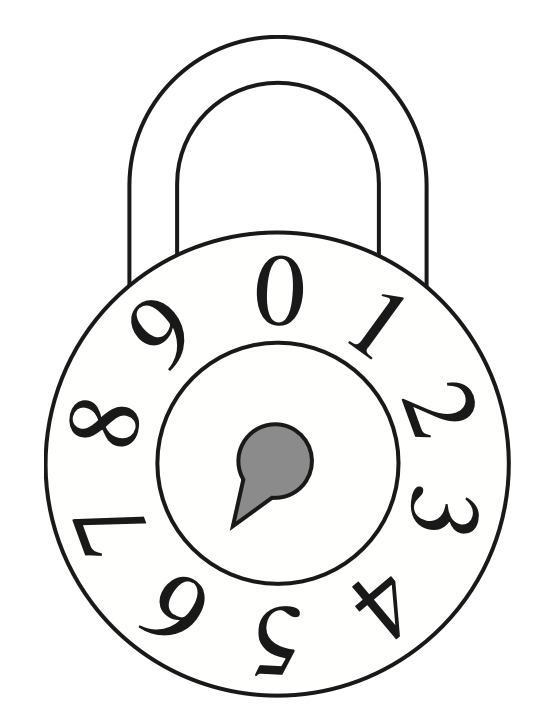
\includegraphics[width=0.12\textwidth]{padlock}
\end{center}
\item Four cards are drawn from a standard deck of 52 cards. In how many ways can this be done if the cards are all of different values (e.g., no two 5s or two jacks) and all of different suits? (For this problem, the order in which the cards are drawn matters, so drawing $A \spadesuit - K \heartsuit - 3 \diamondsuit - 6 \clubsuit$ is not the same as drawing $6 \clubsuit - K \heartsuit - 3 \diamondsuit - A \spadesuit$, even though the same cards are selected.)
\item Let $n$ be a positive integer. Prove that $n^2 = (n)_2 + n$ in two different ways: (1) algebraically, and (2) by list counting.
\end{enumerate}

%--------------------------------------------------------------------
\section*{Factorial (9/14)}
\begin{textbook}{Sec.~9 (Factorial)}
\begin{itemize}[leftmargin=*, nosep]
\item Know how to apply the definition of factorial.
\item Know how to justify why $0!=1$.
\item Understand how to read product notation.
\end{itemize}
\end{textbook}

\begin{enumerate}
\item Your friend Sandy has six different books of classical literature, eight different \textit{romantasy} (i.e.\ romance fantasy) books, and five different self-help books.
\begin{enumerate}
\item In how many different ways can Sandy's books be arranged on a bookshelf?
\item In how many different ways can Sandy's books be arranged on the bookshelf if all books of the same category are grouped together?
\end{enumerate}
\item Evaluate $\frac{100!}{98!}$ without calculating $100!$ or $98!$.
\item Calculate the following products:
\begin{enumerate}
\item $\prod_{k=1}^n \frac{k+1}{k}$. \quad (Reduce this product.)
\item $\prod_{k=1}^n (2k-1)$. \quad (Give an English description.)
\end{enumerate}
\end{enumerate}

%--------------------------------------------------------------------
\section*{Sets (9/16)}
\begin{textbook}{Sec.~10 (Sets)}
\begin{itemize}[leftmargin=*, nosep]
\item Know how to apply the strategy for proving that two sets are equal (Proof Template 5). In particular, know how to prove Prop 10.1.
\item Know how to count the number of subsets of a set.
\end{itemize}
\end{textbook}

\begin{enumerate}
\item Find the cardinality of the following sets
\begin{enumerate}
\item $\set{x \in \mathbb{Z}: |x| \leq 10}$
\item $\set{x \in \mathbb{Z}: 1 \leq x^2 \leq 2}$
\item $\set{x \in \mathbb{Z}: x \in \emptyset}$
\item $2^{2^{\set{1,2,3}}}$
\item $\set{x \in 2^{\set{1,2,3,4}}: |x|=1}$
\item $\set{\set{1,2}, \set{3,4,5}}$
\end{enumerate}
\item Let $A= \set{x \in \mathbb{Z}: 4 \mid x}$ and $B= \set{x \in \mathbb{Z}: 2 \mid x}$. Prove that $A \subseteq B$.
\item Let $A= \set{0,1,2,3,4}$ and $B= \set{x \in \mathbb{N}: x^2<17}$. Prove that $A=B$.
\end{enumerate}

%--------------------------------------------------------------------
\section*{Quantifiers (9/18)}
\begin{textbook}{Sec.~11 (Quantifiers)}
\begin{itemize}[leftmargin=*, nosep]
\item Know how to apply the strategy for proving existential statements (Proof Template 7) to Example 11.1. Know how to apply the strategy for proving universal statements (Proof Template 8) to Example 11.2.
\item Know how to read and negate quantified statements.
\end{itemize}
\end{textbook}

\begin{enumerate}
\item Label each sentence below about the integers as true or false.
\begin{enumerate}
\item $\forall x, \forall y, x+y=0.$
\item $\forall x, \exists y: x+y=0.$
\item $\exists x: \forall y, x+y=0.$
\item $\exists x, \exists y: x+y=0.$
\item $\forall x, \forall y, xy=0.$
\item $\forall x, \exists y: xy=0.$
\item $\exists x: \forall y, xy=0.$
\item $\exists x, \exists y: xy=0.$
\end{enumerate}
\item The notation $\exists!$ can be read ``there is a unique.'' Label each sentence below true or false.
\begin{enumerate}
\item $\exists! x \in \mathbb{N}: x^2=4.$
\item $\exists! x \in \mathbb{Z}: x^2=4.$
\item $\exists! x \in \mathbb{N}: x^2=3.$
\item $\exists! x \in \mathbb{Z}: \forall y \in \mathbb{Z}, xy=x.$
\item $\exists! x \in \mathbb{Z}: \forall y \in \mathbb{Z}, xy=y.$
\end{enumerate}
\item For each sentence below, write the negation of the sentence, but place the $\lnot$ symbol as far to the right as possible. Then rewrite the negation in English. The first problem is done for you.
\begin{enumerate}
\item $\forall x \in \mathbb{Z}, x \text{ is odd.}$ \textit{Solution:} $\exists x \in \mathbb{Z}: \lnot (x \text{ is odd})$. In English: ``There is an integer which is not odd.''
\item $\forall x \in \mathbb{Z}, x<0.$
\item $\exists x \in \mathbb{Z}: x=x+1.$
\item $\exists x \in \mathbb{N}: x>10.$
\item $\forall x \in \mathbb{N}, x+x=2x.$
\item $\exists x \in \mathbb{Z}: \forall y \in \mathbb{Z}, x>y.$
\item $\forall x \in \mathbb{Z}, \forall y \in \mathbb{Z}, x=y.$
\item $\forall x \in \mathbb{Z}, \exists y \in \mathbb{Z}: x+y=0.$
\end{enumerate}
\end{enumerate}

%--------------------------------------------------------------------
\section*{Set Operations (9/21)}
\begin{textbook}{Sec.~12 (Set Operations)}
\begin{itemize}[leftmargin=*, nosep]
\item From Theorem 12.3, know how to prove the associative properties (see text) and distributive properties (see slides).
\item Know how to apply Prop 12.4 (the size of a union) to solve Example 12.5.
\item Know how to prove Prop 12.11 (alternative form of symmetric difference).
\end{itemize}
\end{textbook}

\begin{enumerate}
\item Let $A=\set{1,2,3,4,5}$ and $B=\set{4,5,6,7}$. Please compute (a) $A \cup B$, (b) $A \cap B$, (c) $A - B$, (d) $B-A$, (e) $A \,\triangle\, B$, (f) $A \times B$, and (g) $B \times A$.
\item The distributive properties for sets are
\[ A \cup (B \cap C) = (A \cup B) \cap (A \cup C), \qquad \text{and} \qquad A \cap (B \cup C) = (A \cap B) \cup (A \cap C). \]
The Venn diagram below illustrates the first distributive property. Make a Venn diagram to illustrate the second distributive property.
\begin{center}
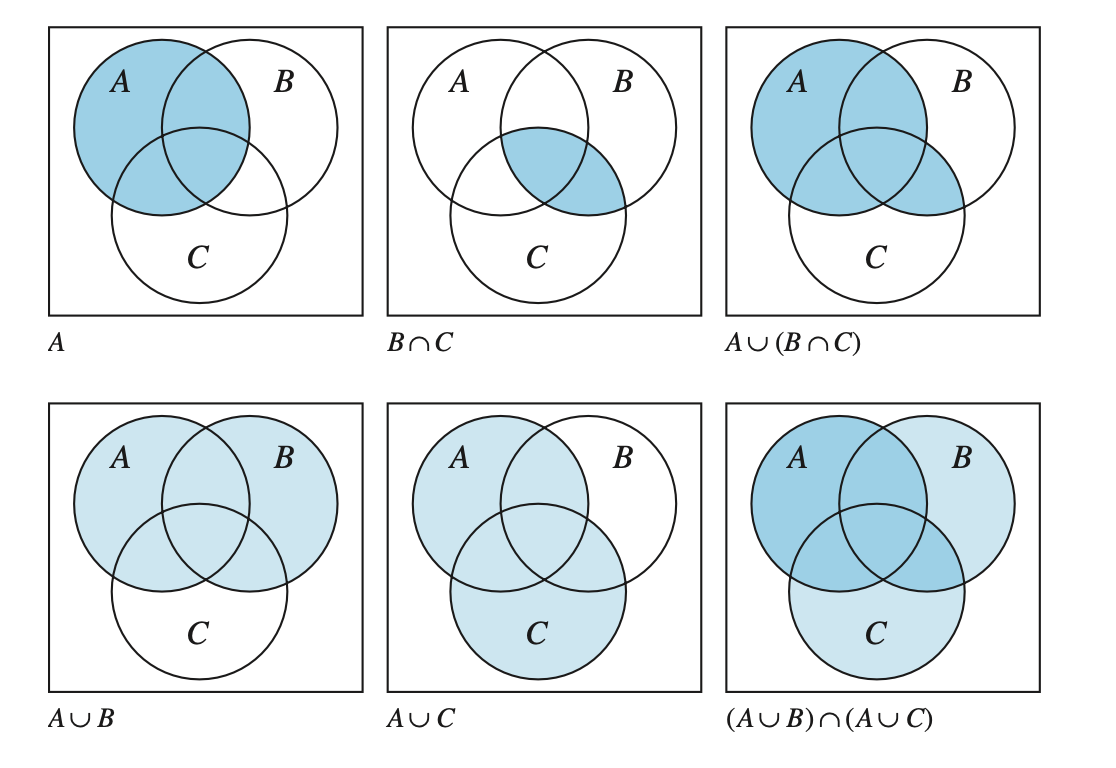
\includegraphics[width=.5\textwidth]{set_distributive_property}
\end{center}
\item Prove that the second identity in \#2 holds. \textit{Hint}: Use Theorem 7.2 (Boolean algebra properties).
\item How many integers in the range 1 to 1000 (inclusive) are divisible by 2 or by 5? Justify your answer. \textit{Hint:} Use Proposition 12.4 (Size of a Union).
\end{enumerate}

%--------------------------------------------------------------------
\section*{Relations (9/23)}
\begin{textbook}{Sec.~14 (Relations)}
\begin{itemize}[leftmargin=*, nosep]
\item Understand the definition of relations in Def 14.2.
\item Know how to determine whether a relation is reflexive, symmetric, and/or transitive, as in Examples 14.8--14.11. (Skip antisymmetric and irreflexive.)
\end{itemize}
\end{textbook}

\begin{enumerate}
\item \textit{(Relations as ordered pairs.)} Write the following relations on the set $\set{1,2,3,4,5}$ as sets of ordered pairs: (a) is-less-than, (b) is-divisible-by, (c) is-equal-to, (d) has-the-same-parity-as. (Note: When we say two numbers have the same parity, we mean they are both odd or both even.)
\item \textit{(Drawing pictures of relations.)} Draw pictures of the following relations on $A$.
\begin{enumerate}
\item Let $A=\set{a \in \mathbb{N} : a \mid 10}$ and let $R$ be the relation $\mid$ (divides) restricted to $A$.
\item Let $A=\set{1,2,3,4,5}$ and let $R$ be the relation $=$ (equals) restricted to $A$.
\end{enumerate}
\item \textit{(Drawing pictures of relations.)} Draw pictures of the following relations on $A \times B$.
\begin{enumerate}
\item Let $A=\set{1,2,3,4}$ and $B = \set{2,3,4}$. Let $R$ be the relation $\geq$ (greater than or equal to) from $A$ to $B$.
\end{enumerate}
\item \textit{(Properties of relations.)} For each of the following relations on the set of all human beings, determine whether the relation is reflexive, symmetric, and/or transitive: (a) is-taller-than, (b) has-the-same-parents-as (i.e., same mother and father), (c) is-the-child-of, (d) is-married-to.
\item \textit{(Properties of relations.)} For each of the following relations defined on the integers, please state whether the relation is reflexive, symmetric, and/or transitive: (a) $=$ (equality), (b) $\leq$ (less than or equal to), (c) $<$ (strict less than), (d) $\mid$ (divides). Please justify your answer for part (d).
\end{enumerate}

%--------------------------------------------------------------------
\section*{Equivalence Relations (9/25)}
\begin{textbook}{Sec.~15 (Equivalence Relations)}
\begin{itemize}[leftmargin=*, nosep]
\item Know how to apply the definition of congruence mod $n$ (to determine whether a pair of numbers is congruent).
\item Know how to prove that congruence mod $n$ is an equivalence relation.
\item Know how to determine equivalence classes as in Examples 15.7 and 15.8.
\end{itemize}
\end{textbook}

\begin{enumerate}
\item Which of the following are equivalence relations?
\begin{enumerate}
\item $\mid$ on $\mathbb{Z}$.
\item $\leq$ on $\mathbb{Z}$.
\item Is-an-anagram-of on the set of English words. (For instance, \texttt{STOP} is an anagram of \texttt{POTS} because we can form one from the other by rearranging its letters.)
\item $R=\set{(1,2),(2,3),(3,1)}$ on the set $\set{1,2,3}$.
\item $\set{1,2,3} \times \set{1,2,3}$ on the set $\set{1,2,3}$.
\item $\set{1,2,3} \times \set{1,2,3}$ on the set $\set{1,2,3,4}$.
\end{enumerate}
\item For each equivalence relation below, find the requested equivalence class(es).
\begin{enumerate}
\item $R=\set{(1,1), (1,2), (2,1), (2,2), (3,3), (4,4)}$ on $\set{1,2,3,4}$. Find $[1],[2],[3],[4]$.
\item $R$ is has-the-same-tens-digit on the set $\set{x \in \mathbb{Z} : 100 < x < 200}$. Find $[123]$.
\item $R$ is has-the-same-parents-as on the set of all human beings. Find [you].
\item $R$ is has-the-same-size-as on $2^{\set{1,2,3,4,5}}$. Find $[\set{1,3}]$.
\end{enumerate}
\item Let $n$ be a positive integer. Prove that congruence modulo $n$ is an equivalence relation on the set of integers.
\end{enumerate}

%--------------------------------------------------------------------
\section*{Partitions (9/28)}
\begin{textbook}{Sec.~16 (Partitions)}
\begin{itemize}[leftmargin=*, nosep]
\item Understand how partitions and equivalence classes are ``two sides of the same coin.''
\item Know how to count the number of ways to rearrange the letters in the words \texttt{WORD}, \texttt{HELLO}, and \texttt{AARDVARK}, and justify your answer using equivalence classes.
\end{itemize}
\end{textbook}

\begin{enumerate}
\item How many different anagrams (including nonsensical words) can be made from each of the following? (a) \texttt{STAPLE}, (b) \texttt{SUCCESS}, (c) \texttt{MISSISSIPPI}.
\item The integers 1 through 25 are arranged in a $5 \times 5$ array (we use each number from 1 to 25 exactly once). All that matters is which numbers are in which column and how they are arranged in the columns. It does not matter in what order the columns appear. (See the figure. The two arrays shown should be considered the same.) How many different such arrays can be formed?
\begin{center}
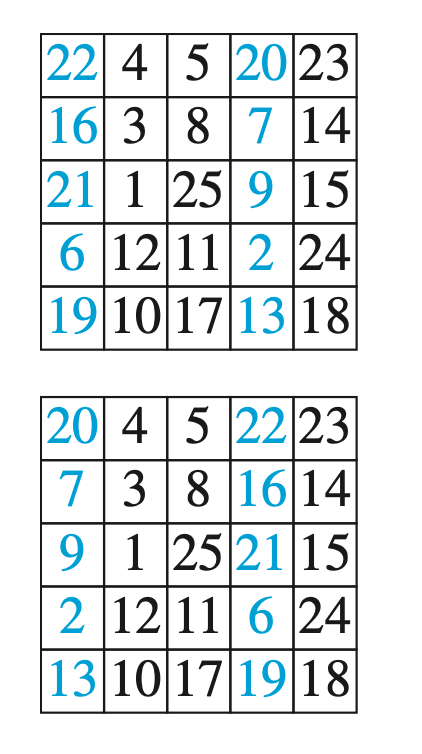
\includegraphics[width=0.18\textwidth]{partition_group_exercise}
\end{center}
\item Twelve people join hands for a circle dance. (a) In how many different ways can they do this? (b) Suppose six of these people are men, and the other six are women. In how many different ways can they join hands for a circle dance, assuming they alternate in gender around the circle?
\end{enumerate}

%%--------------------------------------------------------------------
%\section*{Binomial Coefficients (9/30)}
%\begin{enumerate}
%\item For each question below, determine the answer in three different ways. First, write out all the possible subsets explicitly. Second, use a proposition or theorem from the text. Third, use a different proposition or theorem from the text.
%\begin{enumerate}
%\item Determine the number of 2 element subsets of $\set{1,2,3,4,5,6}$.
%\item Determine the number of 4 element subsets of $\set{1,2,3,4,5,6}$.
%\end{enumerate}
%\item Scheinerman Prop 17.7 says: Let $n,k \in \mathbb{N}$ with $0 \leq k \leq n$. Then
%\[ \binom{n}{k} = \binom{n}{n-k}. \]
%Prove this proposition using Scheinerman Theorem 17.12, which says
%\[ \binom{n}{k} = \frac{n!}{k!(n-k)!}. \]
%\item Fifty runners compete in a 5K race. How many different outcomes are possible? Find different answers according to the context. (a) We want to know in what place every runner finished. (b) The race is a qualifying race, and we just want to pick the ten fastest runners. (c) The race is an Olympic final event, and we care only about who gets the gold, silver, and bronze medals.
%\item At a large community festival, there's a group of 30 volunteers --- 8 from Missoula and 22 from other towns. The organizers want to form a five-person team to plan the main event. However, they insist that at least one person from Missoula must be on the team to make sure the town's voice is heard. How many five-person teams can be formed containing at least one person from Missoula?
%\end{enumerate}

%--------------------------------------------------------------------
\section*{Midterm Review 1: Review of Proofs (10/2)}
\begin{enumerate}
\item Prove that the product of two even integers is even.
\item Let $x$ be an integer. Prove that $0 \mid x$ if and only if $x=0$.
\item Disprove: If $p$ and $q$ are prime, then $p+q$ is composite.
\item Let $A = \set{x \in \mathbb{Z} : 4 \mid x}$ and let $B = \set{x \in \mathbb{Z} : 2 \mid x}$. Show that $A \subseteq B$.
\item Let $A = \set{n \in \mathbb{Z} : 3 \mid n}$ and let $B = \set{n \in \mathbb{Z} : 3 \mid (n+6)}$. Show that $A=B$.
\end{enumerate}

\noindent\fbox{\parbox{\dimexpr\linewidth-2\fboxsep-2\fboxrule}{%
\textbf{Reference: Definitions}
\begin{itemize}
\item Let $a,b$ be integers. We say that $a$ is \textbf{divisible} by $b$, written $b \mid a$, if there is an integer $c$ such that $bc=a$. We call $b$ a \textbf{divisor} of $a$.
\item An integer is called \textbf{even} if it is divisible by 2. (That is, an integer $x$ is even if there is an integer $c$ such that $x=2c$.)
\item An integer $p$ is called \textbf{prime} if $p>1$ and the only positive divisors of $p$ are 1 and $p$.
\item A positive integer $a$ is called \textbf{composite} if there is an integer $b$ such that $1<b<a$ and $b \mid a$.
\end{itemize}}}

\end{document}
